\documentclass[]{article}
\usepackage{lmodern}
\usepackage{amssymb,amsmath}
\usepackage{ifxetex,ifluatex}
\usepackage{fixltx2e} % provides \textsubscript
\ifnum 0\ifxetex 1\fi\ifluatex 1\fi=0 % if pdftex
  \usepackage[T1]{fontenc}
  \usepackage[utf8]{inputenc}
\else % if luatex or xelatex
  \ifxetex
    \usepackage{mathspec}
  \else
    \usepackage{fontspec}
  \fi
  \defaultfontfeatures{Ligatures=TeX,Scale=MatchLowercase}
\fi
% use upquote if available, for straight quotes in verbatim environments
\IfFileExists{upquote.sty}{\usepackage{upquote}}{}
% use microtype if available
\IfFileExists{microtype.sty}{%
\usepackage{microtype}
\UseMicrotypeSet[protrusion]{basicmath} % disable protrusion for tt fonts
}{}
\usepackage[unicode=true]{hyperref}
\hypersetup{
            pdfborder={0 0 0},
            breaklinks=true}
\urlstyle{same}  % don't use monospace font for urls
\usepackage{graphicx,grffile}
\makeatletter
\def\maxwidth{\ifdim\Gin@nat@width>\linewidth\linewidth\else\Gin@nat@width\fi}
\def\maxheight{\ifdim\Gin@nat@height>\textheight\textheight\else\Gin@nat@height\fi}
\makeatother
% Scale images if necessary, so that they will not overflow the page
% margins by default, and it is still possible to overwrite the defaults
% using explicit options in \includegraphics[width, height, ...]{}
\setkeys{Gin}{width=\maxwidth,height=\maxheight,keepaspectratio}
\IfFileExists{parskip.sty}{%
\usepackage{parskip}
}{% else
\setlength{\parindent}{0pt}
\setlength{\parskip}{6pt plus 2pt minus 1pt}
}
\setlength{\emergencystretch}{3em}  % prevent overfull lines
\providecommand{\tightlist}{%
  \setlength{\itemsep}{0pt}\setlength{\parskip}{0pt}}
\setcounter{secnumdepth}{0}
% Redefines (sub)paragraphs to behave more like sections
\ifx\paragraph\undefined\else
\let\oldparagraph\paragraph
\renewcommand{\paragraph}[1]{\oldparagraph{#1}\mbox{}}
\fi
\ifx\subparagraph\undefined\else
\let\oldsubparagraph\subparagraph
\renewcommand{\subparagraph}[1]{\oldsubparagraph{#1}\mbox{}}
\fi

% set default figure placement to htbp
\makeatletter
\def\fps@figure{htbp}
\makeatother


\date{}

\begin{document}

\textbf{BREAKING NEWS: EURO SINDROME NIMBY (sottosezione)}

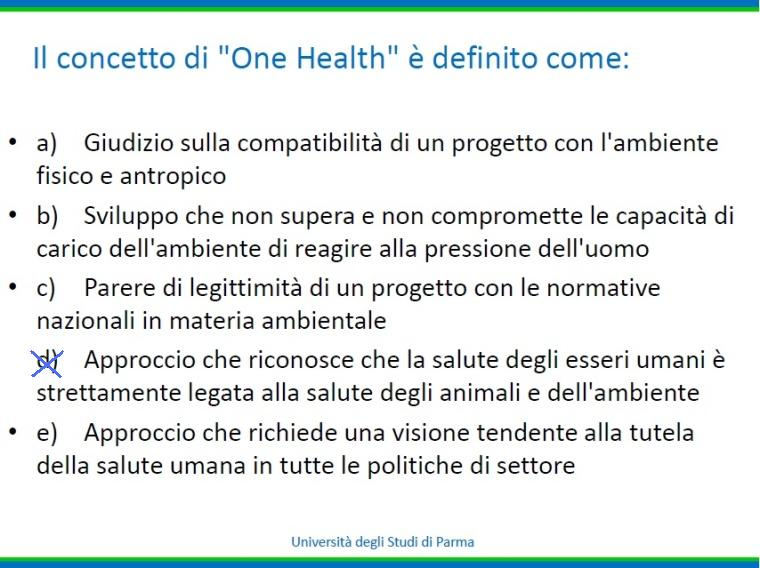
\includegraphics[width=3.85230in,height=2.90990in]{media/image2.emf}

Si inizia con un aneddoto: viene chiesto quanti studenti fanno uso del
profumo Chanel n°5. Diverse mani si alzano.

La nota azienda Chanel sta utilizzando le sue risorse legali per
interrompere i lavori per la costruzione della ferrovia ad alta velocità
Marsiglia-Nizza perché un paio di viadotti andrebbero a distruggere
parte delle coltivazioni di gelsomino, utilizzati nella produzione del
profumo n°5, molto noto e amato.

Questo rientra nel concetto che quando sono presenti delle questioni
ambientali sorgono delle dispute a livello locale che a volte rallentano
i lavori, specialmente per le grandi opere.

Tutti saranno probabilmente d'accordo, Chanel compresa, che la ferrovia
ad alta velocità Marsiglia-Nizza sia utile per tutta una serie di motivi
legati al turismo, all'economia; il difficile è accordarsi sul dove
farla. Sulla strada di questa disputa si può notare come sul Corriere
della Sera dell'altro giorno anche il sindaco di Cannes si sia schierato
con Chanel. Si resta in attesa della risoluzione del conflitto.

Il secondo aneddoto riguarda una disputa tedesca più ``classica'', un
po' meno pittoresca, dove un'azienda nel settore della produzione
dell'energia ha deciso in accordo con il governo di espandere l'area di
utilizzo del sottosuolo per aumentare la produzione di energia. In
questo caso il problema è che si tratta di una foresta di 12mila anni,
con delle riserve di lignite; la disputa riguarda la necessarietà
dell'intervento. È chiaro che si potrebbe scegliere sia una località che
una forma di energia alternativa, per esempio una soluzione potrebbe
essere la costruzione di una centrale nucleare.

Questi sono solo due esempi per concludere ciò che è stato
precedentemente detto; l'importante è che passi il concetto che si
tratta di temi che hanno risvolti indiretti sulla salute, ma che
comunque riguardano una questione ambientale, basti pensare alla
riduzione del traffico che può apportare la costruzione di una ferrovia
ad alta velocità. Lo stesso vale per la questione energetica, la quale è
molto delicata.

Si suggerisce di approfondire i tre argomenti seguenti (clima e aria,
ambienti indoor e rifiuti) in maniera autonoma.

\textbf{CLIMA E ARIA (sezione)}

Per motivi già noti il clima influenza la salute umana.

Questo è noto da oltre due millenni; già in alcuni scritti di Ippocrate
si trattava del rapporto tra ambiente e salute umana.

Studiando le malattie infettive è stato più volte sottolineato come
queste abbiano un andamento che è legata al tipo di clima: l'incidenza è
maggiore normalmente nelle aree calde e umide. È altrettanto noto come i
climi freddi e umidi siano un fattore di rischio per alcune malattie
infettive, soprattutto dell'apparato respiratorio; si ribadisce inoltre
come alcuni aspetti climatici influenzino alcune patologie (come la
depressione, la quale trova nell'aumento dei suicidi il suo punto
estremo) e le abitudini individuali, come l'alimentazione.

È chiaro che l'alimentazione è influenzata dal clima, sia da un punto di
vista psicologico sia per via della disponibilità di alcuni alimenti.
Per esempio in Paesi con climi freddi e rigidi è più difficile reperire
quei cibi cosiddetti ``sani'' tipici ad esempio della dieta
mediterranea; uno dei Paesi dove si mangia peggio in Europa è la
Finlandia. Questo può essere sì dovuto alla presenza di abitudini
individuali particolari, ma è altrettanto importante sottolineare come
sia difficile e dispendioso reperire frutta fresca e verdure (es.
arance) in Finlandia.

Il clima ha quindi un effetto sia diretto che indiretto sulla salute
dell'uomo.

Si invita a soffermarsi in particolare su questi aspetti:

\begin{enumerate}
\def\labelenumi{\arabic{enumi}.}
\item
  ONDATE DI CALORE
\item
  RISCALDAMENTO GLOBALE
\item
  INQUINAMENTO ATMOSFERICO
\end{enumerate}

\textbf{ONDATE DI CALORE (sottosezione)}

Le ondate di calore sono un problema rilevante per la sanità pubblica.
Si tratta di periodi, solitamente di alcuni giorni o di qualche
settimana, spesso nella stagione estiva, dove si raggiungono dei picchi
di temperatura e umidità superiori alla norma che causano una serie di
problemi, soprattutto a determinate fasce della popolazione (ad esempio
persone oltre i 75 anni). Non è specificato, ma sono sicuramente inclusi
anziani che vivono soli e in ambienti caldi e umidi, non adeguatamente
climatizzati.

Cosa può essere fatto per evitare situazioni come nel 2003 quando circa
8000 persone in più rispetto all'andamento normale nel mese di Luglio
sono decedute (morti legate in maniera diretta o indiretta all'ondata di
calore)?

Innanzitutto è importante dare notizia di questi fenomeni; questo perché
spesso nelle grandi città alle ondate di calore corrispondono anche
picchi di inquinamento atmosferico, in particolare da polveri e da
ozono. I consigli alle fasce fragili, che sono quelle in cui si
ritrovano questi 8000 decessi in sovrannumero (quindi over 75, malati
cronici come i cardiopatici e i malati polmonari) sono di:

\begin{itemize}
\item
  \begin{quote}
  evitare lunghe esposizioni esterne
  \end{quote}
\item
  \begin{quote}
  dove possibile controllare il microclima, che è l'elemento
  fondamentale. Se non è presente un climatizzatore può essere
  sufficiente un ventilatore o anche un riscontro d'aria ben fatto tra i
  due affacci di un'abitazione (non è detto che il controllo del
  microclima sia unicamente legato al condizionatore o al
  climatizzatore; se c'è è un vantaggio ma bisogna considerarne i costi
  e il consumo energetico)
  \end{quote}
\item
  \begin{quote}
  alimentazione leggera
  \end{quote}
\item
  \begin{quote}
  abbigliamento idoneo
  \end{quote}
\end{itemize}

Attenzione speciale va riservata anche alle categorie come i neonati o i
pazienti non autosufficienti.

Durante un'ondata di calore si possono avere svariati effetti: caldo,
stress, lipotimia da calore con disorientamento, malessere, debolezza,
nausea, vomito, colpo di calore classico, congestione per bevande
ghiacciate, disidratazione ed effetti e sbalzi pressori.

L'ondata di calore è di per sé un elemento atmosferico che a prescindere
dalle condizioni climatiche aggiunge un fattore di rischio; a volte sono
correlate a fenomeni di inquinamento atmosferico.

\textbf{RISCALDAMENTO GLOBALE ( sottosezione)}

È importante considerare la questione dei cambiamenti climatici in
quanto direttamente collegata all'inquinamento atmosferico: l'aumento
complessivo dell'anidride carbonica nell'atmosfera (dovuta per larga
parte a una maggior quantità di inquinanti atmosferici) porta a quel
fenomeno molto ben conosciuto (e negato, ma da prendere come battuta)
del riscaldamento globale.

Le politiche ambientali sono un tema di dibattito, ma è sicuramente in
corso negli ultimi 50 anni un riscaldamento medio del globo, quindi di
tutta la Terra (riscaldamento globale) misurabile oggettivamente, tant'è
vero che si è osservato un visibile restringimento dei ghiacciai. Questo
è così evidente da essere visibile anche ad occhio nudo; per esempio sul
Monte Bianco sono presenti i segni che mostrano l'altezza che aveva il
ghiacciaio 30 anni fa, rendendo molto facile il confronto con l'altezza
attuale. I ghiacciai si stanno contraendo perché anche una differenza di
mezzo grado è sufficiente per determinare questo fenomeno.

Parallelamente alla contrazione dei ghiacciai esiste motivo di
preoccupazione per l'innalzamento del livello del mare, questo perché
c'è più acqua liquida e meno allo stato solido.

Esistono riscontri diretti sulla salute dell'uomo? Forse, in ogni caso
la questione del riscaldamento globale va necessariamente vista in un
contesto globale di riscaldamento atmosferico per il quale è stata messa
in atto qualche iniziativa, ma che ancora costituisce un problema. Il
famoso protocollo di Kyoto, evocato continuamente, mirava a ridurre i
cosiddetti gas serra (anidride carbonica, metano, protossido d'azoto,
idrofluorocarburi, perfluorocarburi e esafluoruro di zolfo) i quali a
seguito di reazioni chimiche determinano un aumento dell'anidride
carbonica complessiva nell'aria. Da questo deriva il loro nome:
l'effetto serra è così detto perché si fa il parallelo tra quello che
succede nell'atmosfera e quello che succede in una serra d'inverno.
L'anidride carbonica è in grado di catturare radiazioni caloriche; il
suo aumento comporta necessariamente un maggiore intrappolamento quindi
un aumento della temperatura nella troposfera.

Nella serra le radiazioni UV entrano, colpiscono gli oggetti; l'aria
interna si riscalda per conduzione e convezione essendo la serra chiusa:
il calore è in questo modo intrappolato. Questo stesso principio lo si
ritrova nell'atmosfera, con le particelle di CO\textsubscript{2}
responsabili dell'aumento della temperatura.

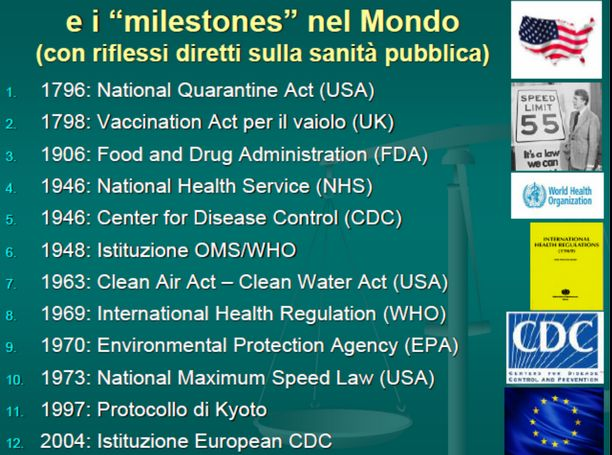
\includegraphics[width=6.64800in,height=2.38687in]{media/image3.emf}

L'effetto serra determina un problema di aumento di temperatura oltre
che di maggior concentrazione degli inquinanti. Perché il problema
dell'inquinamento non è ancora stato risolto nel mondo? Perché il
protocollo di Kyoto è stato pensato e applicato nei Paesi
industrializzati e non in quelli maggiormente problematici oggi,
rispetto a vent'anni fa, come Cina, Brasile ed Est Europa, che oggi sono
i maggiori produttori di inquinamento. Oggi questi Paesi sono economie
emergenti (non è più corretto parlare di Paesi industrializzati e non,
in quanto essi sono oggi realtà industriali assolutamente comparabili se
non superiori a quelle di Europa e Nord America) che non hanno
sottoscritto il protocollo e inquinano molto di più.

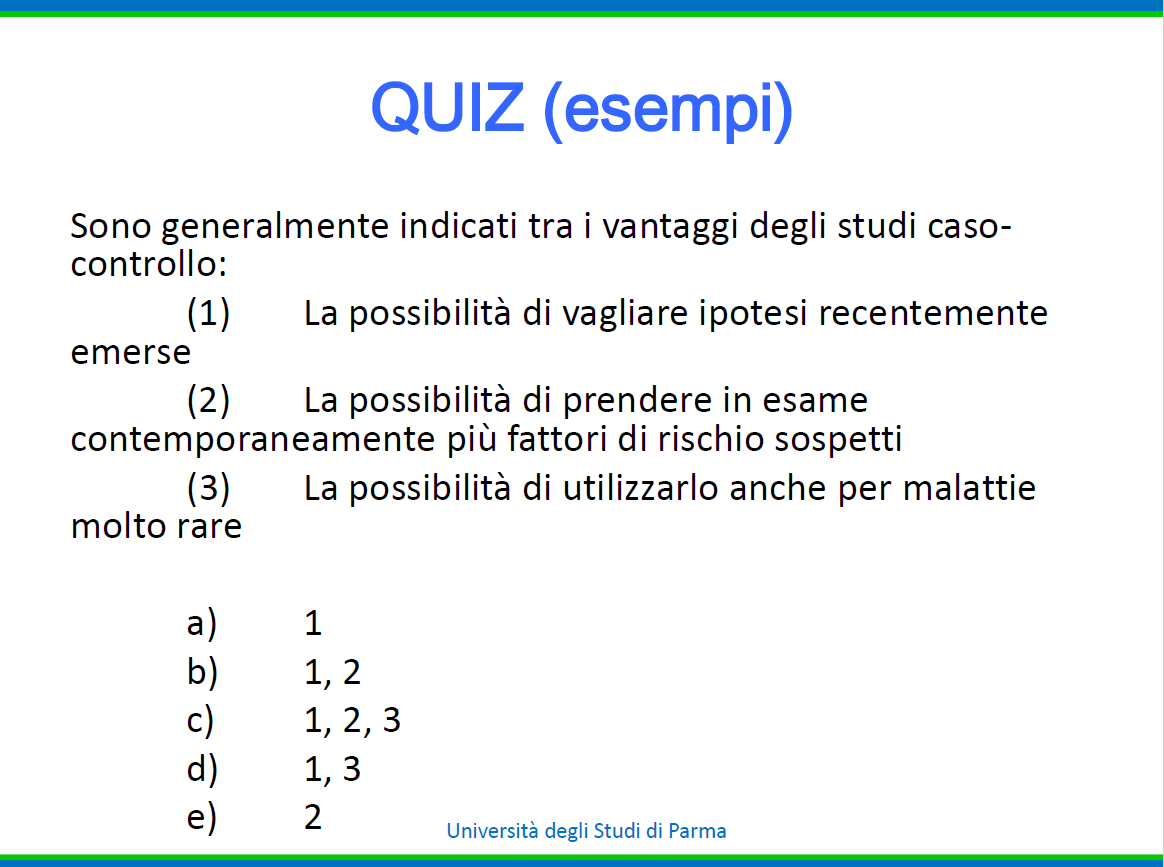
\includegraphics[width=5.61553in,height=3.49311in]{media/image4.emf}

L'atmosfera è però unica: non basta che i Paesi firmatari del protocollo
di Kyoto limitino le loro emissioni, in quanto questo avrà un effetto
solamente parziale se non si convincono in qualche modo i Paesi
precedentemente indicati a seguire modelli di sviluppo più sostenibili,
a riallinearsi, a ridurre questi impatti industriali importanti grazie
alla sottoscrizione di protocolli.

Questo trova una difficoltà nell'applicazione concreta: tutti sono
d'accordo sulla sostenibilità ambientale, ma quando vengono alla luce
gli impatti e le conseguenze economiche pesanti che ha una direzione di
questo tipo è difficile convincere i capi di Governo a sottoscrivere gli
accordi.

Lo sforzo internazionale è in questo momento concentrato su questo
problema.

\textbf{INQUINAMENTO ATMOSFERICO (sottosezione)}

Gli inquinanti atmosferici derivano principalmente, almeno nelle nostre
zone, da tre fonti principali:

\begin{itemize}
\item
  \begin{quote}
  traffico veicolare
  \end{quote}
\item
  \begin{quote}
  impianti termici
  \end{quote}
\item
  \begin{quote}
  impianti industriali
  \end{quote}
\end{itemize}

Queste non sono chiaramente le uniche fonti ma sono le maggiori; le
altre hanno un impatto più ridotto.

La questione dell'inquinamento industriale nell'EU non è ancora
completamente risolta ma è sicuramente molto controllata in quanto
l'Unione Europea ha lavorato su dei limiti di emissione per garantire
soglie precauzionali; oltre a questo tutti i Paesi hanno lavorato per
decentrare gli impianti industriali lontano dalle aree urbane e dai
luoghi abitati.

Per quanto riguarda il traffico veicolare e gli impianti termici, questi
rappresentano le maggiori fonti di inquinamento nelle nostre zone; è
chiaro che per quanto riguarda gli impianti termici esiste un fattore
climatico importante.

Per esempio esistono delle regioni che hanno principalmente o l'uno o
l'altro (alcune entrambi); in Sicilia i ¾ delle case non hanno un
impianto di riscaldamento centralizzato, questo perché le condizioni
climatiche non portano a una reale necessità di riscaldamento, il quale
serve solo alcuni giorni l'anno, qualche settimana al massimo.

In Pianura Padana esiste una norma di legge che limita l'accensione
degli impianti termici nel periodo che va dal 15 ottobre al 15 aprile
con qualche deroga; questi limiti non sono solo legati a una questione
di risparmio energetico ma anche a una questione di immissione nell'aria
di inquinanti. Per esempio a Roma, che è una zona climatica diversa, gli
impianti si accendono il 15 novembre e si spengono il 15 marzo. È
evidente che le città del Nord sommino al traffico veicolare, che c'è
dappertutto, la questione degli impianti termici.

Questo rende ragione del fatto che quando ci sono delle emergenze
inquinamento solitamente si trovano nella stagione invernale, quindi da
novembre a marzo, ad eccezione di alcune situazioni estive che
riguardano soprattutto l'emergenza ozono.

Perché l'inquinamento atmosferico è trattato alla Facoltà di Medicina?
Perché ha un effetto provato sulla saluta umana; è necessario utilizzare
la dovuta circospezione nel maneggiare le stime e gli studi, ma che un
effetto ci sia è innegabile. Viene stimata una riduzione della durata
della vita di circa 8 mesi e mezzo per chi vive in aree inquinate
rispetto a chi vive in aree non inquinate: si parla quindi di una
aspettativa di vita minore di circa un anno legata a problemi di
inquinamento atmosferico.

Esiste però una buona novità: il piombo, lo zolfo, il monossido di
carbonio e gli idrocarburi negli ultimi 30 anni si sono ridotti grazie
agli interventi, alle misure, ai nuovi limiti di legge creati; c'è
quindi un leggero miglioramento della situazione. A questo miglioramento
però sono state comunque associate delle restrizioni in termini di
concentrazione perché negli anni sono via via usciti diversi studi
scientifici che hanno dimostrato che anche i livelli precedentemente
ritenuti di sicurezza in realtà aggiungono dei rischi: esiste una
relazione dose -- effetto tra l'esposizione all'inquinamento e la salute
umana.

Tutt'oggi si hanno i problemi relativi alle \emph{polveri sottili},
all'\emph{ozono}, all'\emph{azoto} legati soprattutto ai motori delle
auto e dei mezzi diesel. La stima è di 350.000 decessi annui dovuti
all'inquinamento atmosferico. Questi problemi sono sia acuti
(aggravamento dell'asma, diminuzione della funzione polmonare, effetti
sull'apparato cardiovascolare) sia cronici legati più che altro alla
patologia tumorale e alle BPCO. È bene ricordare come l'interazione tra
più inquinanti e il fumo di sigaretta (che poi sprigiona le stesse
sostanze contenute nell'atmosfera ma il cui effetto è chiaramente
maggiore) determini questi eccessi di rischio che portano a quegli
aumenti di patologia cronica.

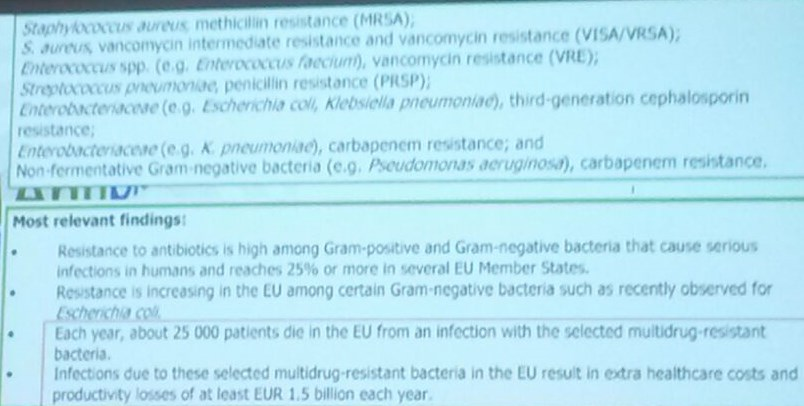
\includegraphics[width=6.47132in,height=4.96104in]{media/image5.emf}

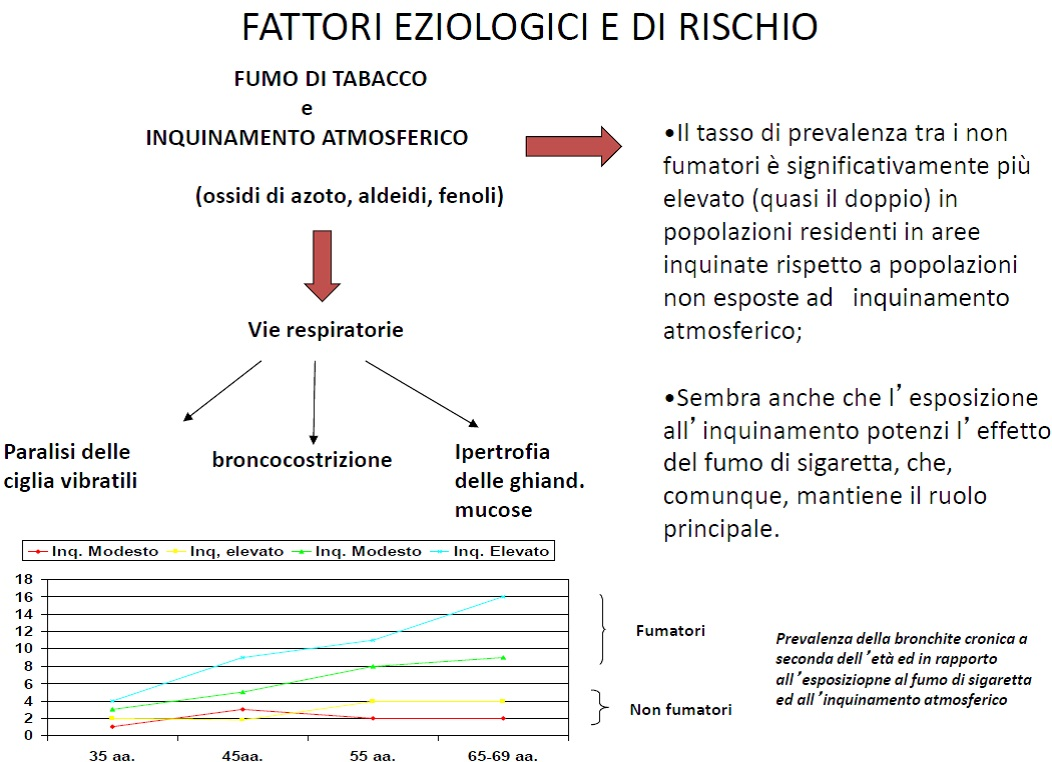
\includegraphics[width=6.40238in,height=4.63793in]{media/image6.emf}

La stima precedentemente nominata è stata recentemente alzata a 467.000
morti annue dall'agenzia della UE che si occupa di ambiente. Le zone
dove c'è più particolato sottile sono le zone europee dove c'è un
maggior inquinamento atmosferico.

Si osservi come in questo momento una delle aree ad altissimo rischio
sia la Pianura Padana, questo per un fatto geografico (si parla di
\emph{cul de sac}: è una regione chiusa a nord dalle Alpi e dalle
Prealpi, a sud dall'Appennino con un solo sbocco sul mare che è
l'Adriatico); le altre sono aree est europee, in particolare la Polonia,
la Bulgaria e la Romania. Il problema è minore in Francia, in Germania e
in Spagna. I dati forniti sono basati sulla osservazione annuale.

La situazione della Pianura Padana è particolarmente grave perché la sua
conformazione e la mancanza di sbocchi portano a un ristagno degli
inquinanti che porta a un fenomeno di inversione termica, con ricaduta
al suolo degli stessi; ciò comporta per alcuni giorni all'anno una
situazione abbastanza critica che non riguarda più soltanto le grandi
città. Quando gli inquinanti sono imprigionati dai fenomeni di
inversione termica hanno una ricaduta al suolo a prescindere dalla aree
in cui si hanno emissioni o meno.

Tuttavia, con qualche picco variabile di anno in anno, negli ultimi
dieci anni sono in calo i giorni in cui vengono superati i limiti
stabiliti dalla normativa europea come pericolosi per la salute
dell'uomo; in sostanza i provvedimenti presi, soprattutto nel settore
delle auto e del trasporto motorizzato, hanno sortito qualche effetto.
Questo non è sufficiente per stare tranquilli, però è comunque un
segnale di miglioramento. È bene notare che nelle aree dove è possibile
un maggior ricircolo dell'aria, anche nei giorni di superamento
l'inquinamento atmosferico è minore perché c'è una dispersione degli
inquinanti (es. Como città sul lago è dotata di maggiore areazione). È
però presente a livello di regione una situazione del tipo
precedentemente descritto.

La prevenzione dell'inquinamento atmosferico è un argomento già
conosciuto e trattato, è qualcosa di cui si sente parlare tutti i
giorni, è sufficiente aprire i giornali d'inverno e si può leggere di
casi del genere.

La prevenzione dell'inquinamento industriale, come già sottolineato, è
basata sullo smaltimento degli inquinanti e sulla delocalizzazione delle
aree; per quanto riguarda il traffico motorizzato esistono restrizioni
sulla circolazione dei mezzi, divieti, riduzione dei mezzi dove
possibile, scorrimento e parcheggi, uso di combustibili ecologici,
mobilità sostenibile: tutto ciò è ovvio ma non semplice da realizzare
nella pratica e in ogni luogo. Per quanto riguarda gli impianti termici
resta ancora molto da fare, non perché non sia già in corso un
efficientamento degli impianti ma perché vi è una componente individuale
più importante che è quella della regolazione della temperatura, che
determina i consumi e quindi influisce non solo sul risparmio energetico
ma anche sull'inquinamento. Qui purtroppo le leggi non possono essere
più di tanto efficaci: è vero che esistono dei limiti di temperatura
negli ambienti che devono essere rispettati ma di fatto è necessario
affidarsi al buonsenso delle persone che devono, laddove possibile,
cercare di limitare i consumi. Chiaramente in alcuni casi l'impianto è
centralizzato quindi la regolazione non spetta al singolo.

Una nuova norma ha imposto i controlli per ogni impianto termico di ogni
unità immobiliare: questo viene fatto negli edifici di nuova
costruzione. Per quanto riguarda le strutture più datate questa è
un'operazione più lenta perché bisogna considerare la situazione
italiana; in Italia infatti si ha un patrimonio immobiliare magari di
pregio, ma molto antico quindi gli interventi sul patrimonio immobiliare
già esistente sono più difficoltosi rispetto alle nuove unità
immobiliari.

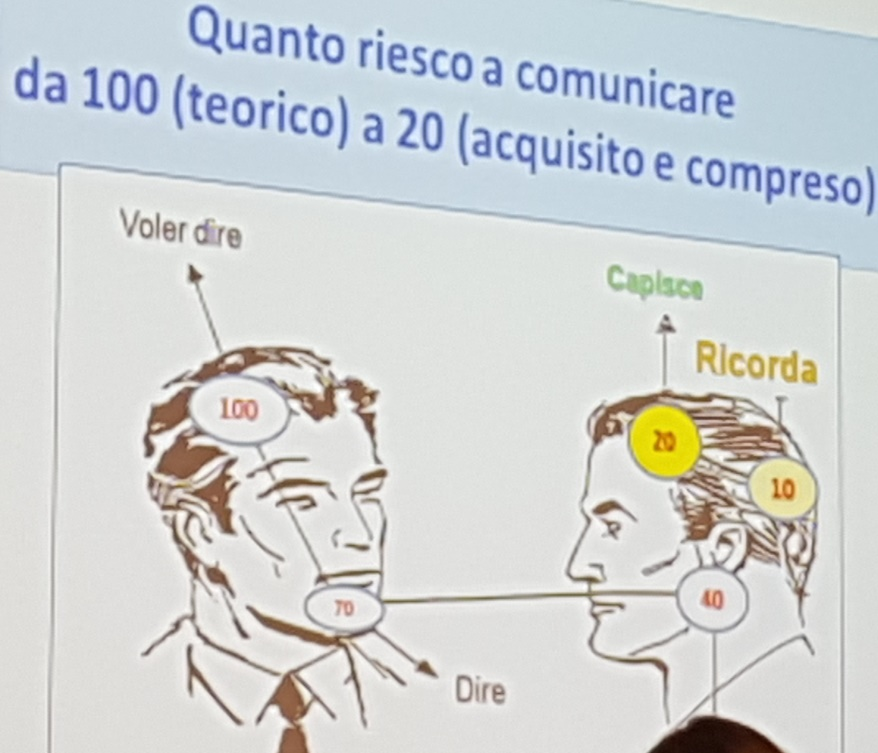
\includegraphics[width=5.25529in,height=3.47015in]{media/image7.emf}

Oltre ai sopracitati interventi, sono interessanti i suggerimenti che il
medico può dare al singolo cittadino:

\begin{itemize}
\item
  \begin{quote}
  controllo della temperatura degli ambienti domestici
  \end{quote}
\item
  \begin{quote}
  verifiche puntuali degli scarichi dei veicoli
  \end{quote}
\item
  \begin{quote}
  evitare attività fisiche in aree inquinate. Si parla di tempo di
  esposizione, vulnerabilità personale e pericolosità delle sostanze.
  Iperventilando si respira una quantità d'aria maggiore: se l'aria è
  inquinata chiaramente si respirerà anche una quantità di inquinanti
  maggiore. Per questo motivo è sconsigliabile andare a fare jogging o
  in bicicletta in aree inquinate.
  \end{quote}
\end{itemize}

Per quanto riguarda il problema dell'ozono si suggerisce di approfondire
l'argomento a casa. L'ozono è un inquinante secondario, per la cui
formazione sono necessarie tre condizioni:

\begin{itemize}
\item
  \begin{quote}
  presenza di precursori, gli ossidi d'azoto, sempre presenti
  \end{quote}
\item
  \begin{quote}
  presenza di sostanze organiche anche di origine naturale, che si vanno
  a combinare con gli ossidi d'azoto
  \end{quote}
\item
  \begin{quote}
  presenza di radiazione ultravioletta, necessaria per la reazione
  chimica; non a caso si parla di smog fotochimico.
  \end{quote}
\end{itemize}

Quand'è che si verificano queste tre condizioni? Gli ossidi d'azoto sono
sempre presenti; le sostanze naturali che si combinano con gli ossidi
d'azoto sono nell'atmosfera, per assurdo, più nelle zone ``verdi'' che
nelle zone abitate, perché vengono rilasciate da vegetali; i raggi UV ci
sono quando c'è molto sole quindi nella stagione estiva. Questo comporta
quindi che l'ozono raggiunga livelli elevati d'estate, in particolare
modo nelle ore centrali più soleggiate, non necessariamente nelle aree
urbane: per esempio sull'Appennino si troveranno alti livelli d'ozono,
così come sulle Prealpi ecc. Nelle giornate di vento l'ozono avrà invece
dei livelli minori perché i precursori vengono a mancare: c'è una
maggior dispersione di questi nell'aria.

L'inquinamento da ozono si distingue quindi da tutti gli altri
inquinamenti (come la polvere, gli ossidi d'azoto, polveri di zolfo e
idrocarburi) perché non si trova necessariamente vicino alla fonte di
emissione ma anche lontano da essa.

Le piccole precauzioni che si possono prendere sono per esempio di
utilizzare la funzione ricircolo dell'aria quando si è in macchina fermi
con il motore acceso per evitare di respirare lo scarico del veicolo che
precede; si tratta chiaramente di qualcosa di ovvio e rientra nella
prevenzione per avere stili di vita più salutari e sostenibili.

\textbf{INQUINAMENTO INDOOR (sezione)}

Il problema dell'aria inquinata è un problema che riguarda sia gli
ambienti outdoor ma anche quelli indoor. Se è inquinato fuori, è anche
inquinato dentro.

Se per esempio si considerano le case tipiche di San Francisco o
\emph{le detached/semi detached houses} londinesi (case di uno/due piani
che possono trovarsi affacciate su delle vie molto frequentate con
incolonnamenti) all'interno delle abitazioni si ritroveranno dei livelli
di inquinamento atmosferico molto simili a quelli esterni.

Se invece consideriamo la vita all'ottantesimo piano di un grattacielo
avremo altri problemi ma comunque non legati all'inquinamento dell'aria.

San Francisco si trova in una baia, quindi è molto ventosa e poco
indicata da portare come esempio per l'inquinamento atmosferico. Invece
Los Angeles, sempre in California, avendo delle catene montuose
abbastanza vicine, è soggetta a un fenomeno che si chiama inversione
termica da stasi dove c'è un imprigionamento degli inquinanti in un'area
che non è troppo vasta e che è sostanzialmente l'area metropolitana di
LA. Questo è un problema che era già presente negli anni Settanta ed è
stato in parte risolto, sostanzialmente cambiando nell'arco di 10 anni
tutto il parco veicolare. Essendo in America il petrolio a basso costo,
la tendenza è quella di circolare con delle macchine di grossa
cilindrata che consumano molto; hanno quindi ridotto il parco veicolare
con ragionevole rapidità e hanno in questo modo parzialmente risolto.

L'inquinamento indoor è riferito per definizione ad ambienti di vita e
lavoro (non industriale): abitazioni, uffici, strutture comunitarie,
locali destinati ad attività ricreative, mezzi di trasporto pubblici o
privati.

Esiste una letteratura che illustra quali possono essere i problemi
legati ad ambienti confinati, dove tutti trascorrono una parte
importante del tempo. Per quanto riguarda la professione medica (noi) la
tendenza è di passare circa il 90-95\% del proprio tempo in ambienti
indoor; di questo totale il 55\% è trascorso nella propria abitazione. È
necessario includere nel conto le ore di sonno e le ore passate a casa a
svolgere diverse attività. Queste percentuali cambiano a seconda della
professione: il lavoratore stradale (es. vigile urbano, fattorino ecc)
passerà almeno 8 ore giornaliere in un ambiente esterno (queste
professioni sono comunque una percentuale piuttosto bassa).

Considerando queste percentuali è chiaro capire che se si parla di
salute è sì interessante l'inquinamento atmosferico (se ne sono viste le
implicazioni sull'ambiente, sulla temperatura terrestre ecc) però è
altrettanto importante considerare gli ambienti confinati nei quali di
fatto si trascorre una quantità importante del proprio tempo.

Quali sono gli elementi da considerare?

\begin{itemize}
\item
  \begin{quote}
  temperatura dell'aria
  \end{quote}
\item
  \begin{quote}
  umidità relativa
  \end{quote}
\item
  \begin{quote}
  calore radiante
  \end{quote}
\item
  \begin{quote}
  velocità dell'aria
  \end{quote}
\item
  \begin{quote}
  illuminazione
  \end{quote}
\item
  \begin{quote}
  rumore
  \end{quote}
\item
  \begin{quote}
  sicurezza
  \end{quote}
\item
  \begin{quote}
  benessere visivo
  \end{quote}
\item
  \begin{quote}
  odori; se derivati da inquinamenti possono avere un significato anche
  diretto per quanto riguarda i problemi della salute. Ci sono odori che
  non hanno effetti sulla salute fisica ma che disturbano, interferendo
  con la salute intesa come benessere mentale e sociale, altrettanto
  fondamentale.
  \end{quote}
\end{itemize}

Si considerino quindi alcuni elementi, come l'\textbf{illuminazione} e
il \textbf{benessere visivo}.

Il benessere visivo è importante. Per esempio una quindicina di anni fa
ci fu una disputa accesa che vide interessata l'AUSL, la quale ha un
ruolo nello stabilire le regole di idoneità degli alloggi, ed
eventualmente intervenire laddove ci siano condizioni di vita non idonee
negli ambienti confinati.

Le regole abitative sono ancora stabilite dai regolamenti comunali.
Circa 15 anni fa in tutte le grandi città si fece il recupero dei
sottotetti al fine di recuperare volumetrie non utilizzate. Considerando
un'unità immobiliare ricavata nel sottotetto, possono insorgere problemi
come quello dell'illuminazione, per esempio se il tetto è chiuso. Questo
però è facilmente risolvibile in quanto la tecnologia oggi ci mette a
disposizione delle aperture fenestrate di qualsiasi dimensione,
impermeabili e di facile installazione, senza il bisogno di cambiare il
tetto: i famosi lucernari.

Una regola generale stabilisce che è necessario avere una superficie
fenestrata in proporzione di 1/8 rispetto alla superficie calpestabile
(con qualche eccezione, ma in generale per una stanza di otto metri
quadrati è necessario considerare almeno un metro quadrato di finestra).

Nel caso dei sottotetti il problema non riguarda le dimensioni adeguate
della finestra, anche perché si ha il vantaggio di non avere ostacoli;
si pensi invece a un primo piano in cui magari, anche se la finestra
c'è, la luce viene parzialmente sottratta dall'ombra di un altro
edificio, quindi la luce naturale che arriva è minore. Le case ai piani
bassi sono di solito meno illuminate rispetto agli ultimi piani dove
l'illuminazione è garantita. Ipotizziamo però che in quest'ultimo piano
abiti un anziano: esce poco di casa e guardando fuori dalle finestre non
vedrà altro che cielo (che tra l'altro in Pianura Padana non è neanche
il massimo). Tutto questo per sottolineare il fatto che il benessere
visivo è importante e l'AUSL della città di Milano aveva imposto quindi
di non creare soltanto lucernari perché questi non lo garantivano. Il
risultato fu che i costruttori inventarono una soluzione tecnica
denominata ``uscita a cappuccino'', cioè dei tagli nel tetto con
sporgenze che garantissero la finestra orizzontale, quindi degli aggetti
che escono e che cambiano la conformazione dell'edificio, soddisfacendo
la condizione di benessere visivo dall'interno. Questo però aveva anche
l'effetto di influire notevolmente sull'impatto visivo dall'esterno,
peggiorando notevolmente l'aspetto precedente del tetto, più compatto,
anche con delle finestre tipo lucernari che non rovinavano l'impatto
soprattutto nelle aree di pregio come i centri storici.

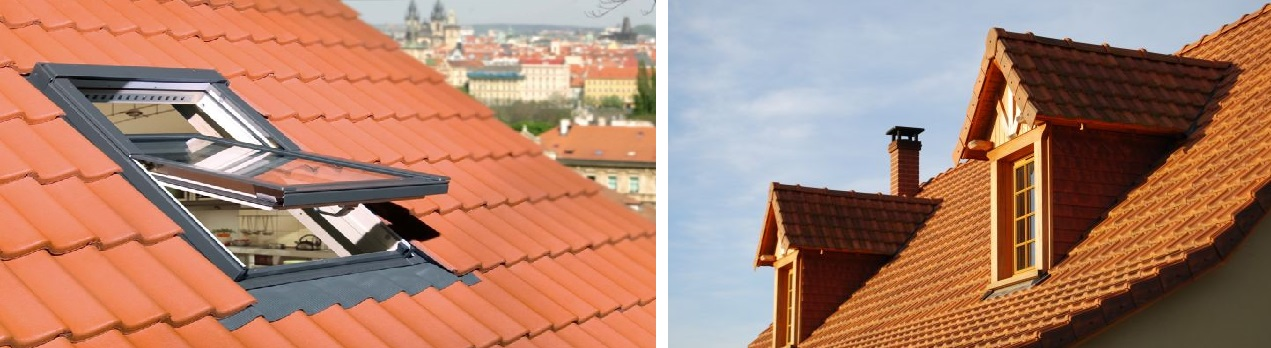
\includegraphics[width=6.75961in,height=1.84800in]{media/image8.jpeg}

Questo sfruttamento dei sottotetti ha quindi impattato sul benessere
visivo della comunità.

E' chiaro che l'illuminazione naturale è importante in alcuni locali
dove si trascorre la maggior parte del tempo, come le abitazioni; è meno
importante in locali dove invece si passano meno ore, come un'aula. Non
lo è per niente, anzi può essere problematico, in alcuni locali
ospedalieri come le sale operatorie dove comunque la luce naturale non
sarebbe sufficiente per soddisfare le esigenze di illuminazione del
campo operatorio e in più potrebbe determinare abbagliamento. È quindi
indifferente per una sala operatoria avere o meno una finestra, anzi si
cercano soluzioni differenti, sia per la mancata utilità sia perché
appunto non soddisfa i requisiti di illuminazione richiesta. Per un'aula
il discorso è invece diverso; ad ogni modo il concetto è che ogni locale
ha la sua regola e laddove è necessario è importante garantire una
quantità nei termini di 1/8 di superficie dedicata.

Un altro problema che riguarda i locali confinati è il \textbf{ricambio
d'aria}; questo è importante e ciascun locale ha delle esigenze diverse.
Nelle abitazioni si ha poca necessità di ricambio d'aria in quanto in
esse normalmente abitano poche persone; la densità è quindi piuttosto
bassa e normalmente, con la sola eccezione della cucina, non sono
presenti inquinanti. È diverso invece per un ambiente come un'aula, dove
devono essere presenti delle cubature minime e dei ricambi minimi;
queste saranno maggiorate negli ambienti con produzione di odori e
calori come bagni, cucine (soprattutto commerciali). Si passa dai 15
ricambi all'ora necessari per legge nelle sale operatorie ospedaliere
(il motivo è la presenza dei gas anestetici che devono essere evacuati
velocemente per non causare problemi al personale) per arrivare ai 30
ricambi orari in quei locali confinati dove è possibile fumare (legge
Sirchia, che aveva vietato il fumo in tutti i locali pubblici). I
locali-ristorante lo hanno fatto all'inizio per poi di fatto
abbandonarlo velocemente: avere 30 ricambi orari in un locale confinato
significa avere una costante corrente d'aria piuttosto fastidiosa. A
volte negli aeroporti ci sono delle sale per fumatori dove
effettivamente vengono garantiti i 30 ricambi all'ora, il minimo
richiesto dalla legge per consentire il fumo all'interno di un luogo
confinato aperto al pubblico in Italia. È chiaro che a casa propria
ognuno è libero di fare quello che crede, però con una forte
raccomandazione quando ci sono i bambini per evitare di fumare in casa
quando sono presenti, perché il danno da fumo passivo è molto maggiore
nei soggetti più fragili.

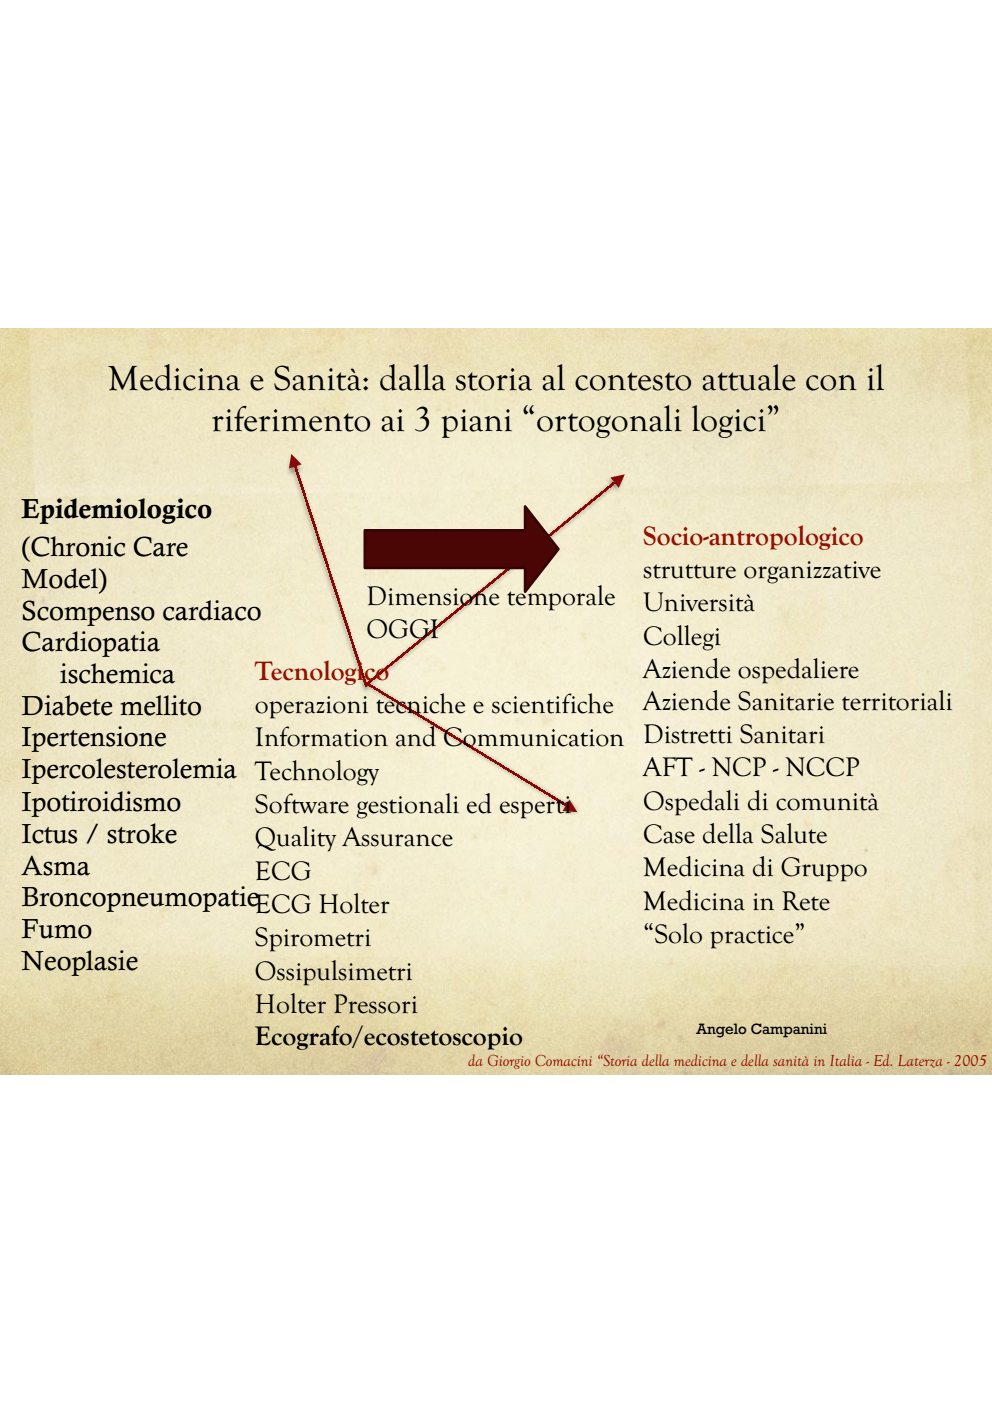
\includegraphics[width=5.19896in,height=2.57669in]{media/image9.emf}

Come avvengono i ricambi d'aria negli ambienti confinati?

\begin{itemize}
\item
  spontaneamente: soluzione di continuo di porte/finestre
\item
  aprendo porte e finestre
\item
  con sistemi artificiali: aspirazione, ventilazione meccanica fino ad
  arrivare al condizionamento dell'aria
\end{itemize}

È chiaro che nelle soluzione abitative sono sufficienti forme di
ricambio naturali; nei locali invece ad uso pubblico è quasi sempre
indispensabile utilizzare forme di ventilazione meccanica.

È importante considerare come nei nostri climi dal punto di vista
energetico sia più conveniente un impianto di ricambio d'aria meccanico
che non l'apertura periodica di porte e finestre; non è un caso che
tutta l'edilizia alberghiera recente non costruisca più porte e finestre
che si aprono nelle camere per non lasciare la discrezionalità al
cliente di aprire e disperdere energia. Negli alberghi la tendenza
adesso è di creare dei sistemi di ventilazione meccanica che consentano
il condizionamento e la climatizzazione che garantiscano minori costi,
perché aprire la finestra significa creare una dispersione molto più
costosa in termini energetici di una ventilazione meccanica costante.

L'unica eccezione, negli alberghi di recente costruzione, si può trovare
nelle località marine dove l'apertura di porte e finestre può avere un
significato diverso.

Più il clima è rigido più diventa importante \textbf{la tenuta degli
infissi} che ha un duplice connotato: da un lato porta a un risparmio
energetico, dall'altro diminuisce i ricambi d'aria. Laddove c'è
l'impianto a tenuta occorre calcolare bene (compito dei
progettisti/impiantisti ) i ricambi d'aria.

Perché è necessario avere ricambi d'aria in ambienti confinati? Per via
dell'accumulo di eventuali patogeni o polveri sottili o anche di gas
nocivi (per esempio in alcuni scantinati). Oltre a questo è fondamentale
ricordare che i ricambi sono necessari perché si respira aria a
temperatura e umidità ambientali, ma la si espira a 36°C e satura, con
il 100\% di umidità. Se in un ambiente confinato sono presenti persone
(e più sono più chiaramente la condizione peggiora) in poco tempo e
senza ricambi d'aria si ha una situazione di aumento della temperatura e
dell'umidità, senza considerare gli odori che sono un'altra
caratteristica da tenere presente negli ambienti confinati.

Se questo avviene nella propria camera è superabile; nel momento in cui
si parla di locali pubblici è invece opportuno intervenire con i dovuti
ricambi d'aria.

Allontanare gli inquinanti quando presenti è altrettanto importante
(ricordare l'esempio della sala operatoria); possono essere infatti
presenti sostanze tossiche o che danno degli effetti. In una cucina si
ha, oltre ai cattivi odori, una concentrazione di monossido di carbonio
maggiore; nei bagni invece avremo principalmente il problema dei cattivi
odori e i ricambi d'aria assumono il significato di garantire il
completo benessere della persona.

Unendo quindi la questione del microclima e degli inquinanti bisogna
considerare anche l'aspetto minoritario della presenza di agenti
biologici. Il problema non è tanto la presenza di meningococchi
nell'aria, ma i contatti diretti: è quindi importante non affollare
eccessivamente i luoghi confinati più che il ricambio d'aria. Per
impedire lo scambio di microrganismi sono più importanti dispositivi di
tipo individuale come il lavaggio delle mani, non tossire o starnutire
che sono modi per trasmettere le malattie a trasmissione aerea.

I parametri ottimali da soddisfare per stare bene sono:

TEMPERATURA: inverno tra i 19° e i 22°C (tant'è che una legge datata ma
ancora vigente afferma che in casa la massima è di 20° C con una
tolleranza di più o meno 2°C);

UMIDITA': tra il 40-60\%; se l'aria è troppo secca o troppo umida si
possono avere dei problemi alle alte vie aeree (problemi di irritazioni
o anche infettivi);

MOVIMENTO DELL'ARIA: avrà un effetto positivo o negativo a seconda della
situazione; d'estate è un piacere, d'inverno peggiora la situazione
microclimatica delle persone.

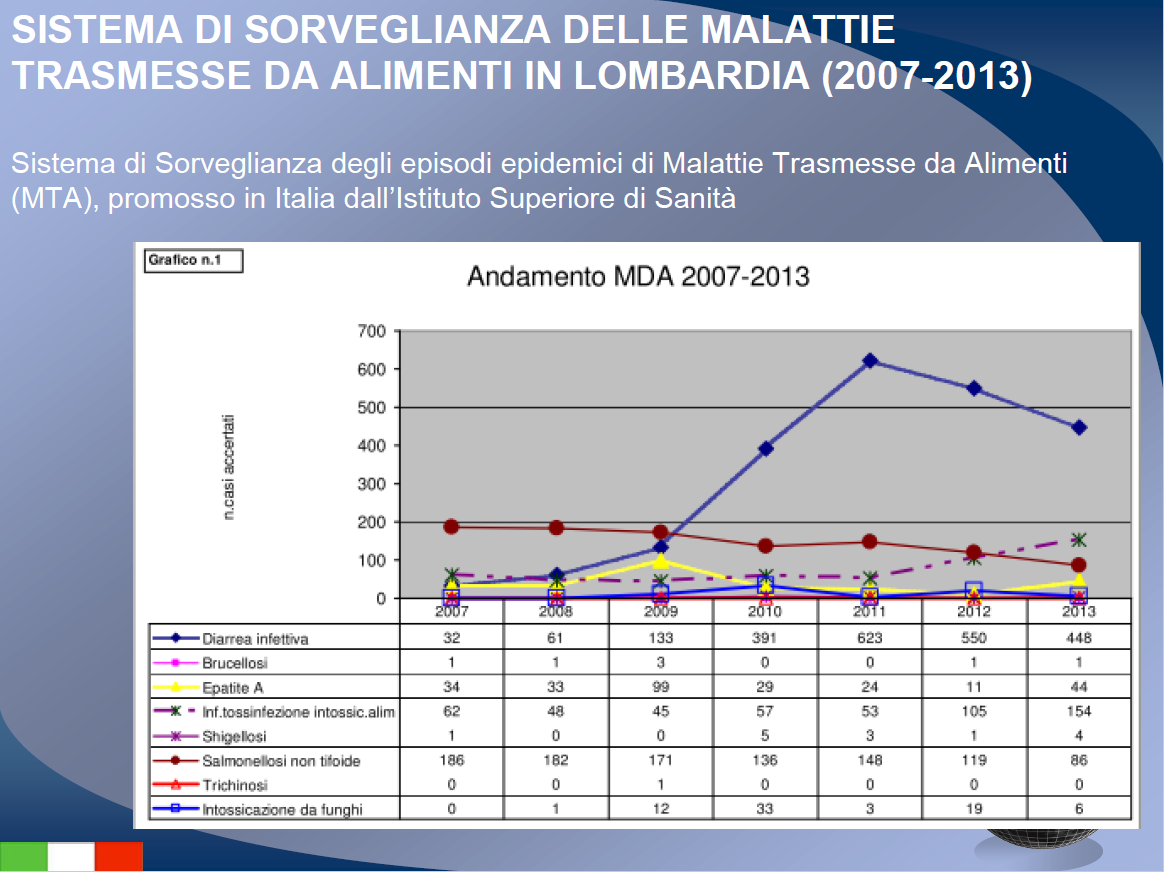
\includegraphics[width=5.86260in,height=3.01841in]{media/image10.emf}

La precisazione della differenza tra estate e inverno è doverosa perché
si utilizza generalmente un vestiario diverso e quindi nella stagione
estiva sono tollerati valori di temperatura più alti, insieme a un po'
di umidità.

Normalmente si ha un'area di benessere che non ha un valore fisso ma è
dato da alcune combinazioni che garantiscono lo stare bene; queste
combinazioni sono anche legate a fattori individuali, al punto che non
ci sono condizioni microclimatiche ottimali e che in qualunque
condizione ci sarà sempre qualcuno che non è in una situazione di
comfort; è per questo motivo che è importante influenzare con il
vestiario il proprio stato di maggiore o minore benessere.

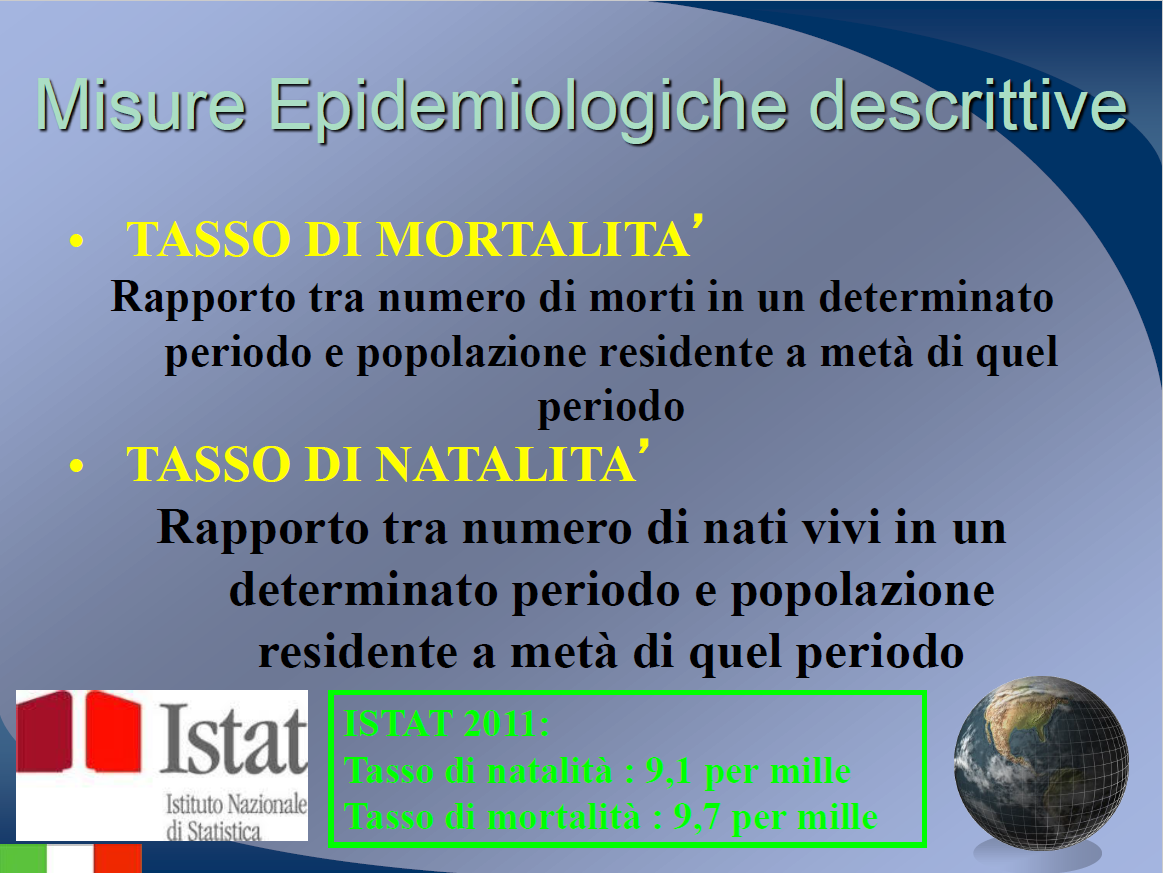
\includegraphics[width=6.08960in,height=3.15781in]{media/image11.emf}

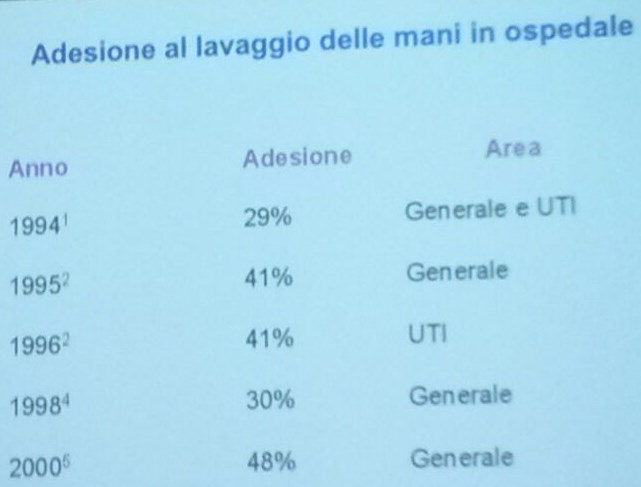
\includegraphics[width=5.75000in,height=2.88490in]{media/image12.emf}

Per concludere (con la raccomandazione di leggere autonomamente questa
parte) si elencano gli inquinanti indoor più importanti:

AGENTI BIOLOGICI: microrganismi, batteri e virus soprattutto, oltre che
allergeni che possono causare problemi alla salute umana

AGENTI FISICI: le radiazioni, il radon

AGENTI CHIMICI: sono la stragrande maggioranza: ossido di azoto,
monossido di carbonio, composti organici volatili, fumo di tabacco,
idrocarburi, anti parassitari, amianto, fibre minerali sintetiche ecc.
Questi agenti sono rilevanti non tanto per le abitazioni quanto per i
locali adibiti a scopo lavorativo (il corso di Medicina del Lavoro avrà
sicuramente trattato tutti gli inquinanti presenti nei locali sia
confinati che non confinati).

Quando si parla di benessere negli ambienti confinati è fondamentale non
fermarsi al benessere fisico come assenza di malattia, ma considerare
anche gli altri aspetti che contribuiscono al benessere mentale e
sociale dell'individuo evocato dall'inizio del corso. Si devono
considerare quindi anche aspetti come tutela della privacy, visione del
paesaggio esterno, sistema del verde, clima cromatico, dimensione e
proporzionalità, sensazione di sicurezza; questi sono tutti elementi che
incidono sul benessere della persona, alcuni in misura maggiore e altri
in misura minore.

Si rimanda alle lezioni precedenti per ulteriori informazioni. Negli
ambienti confinati oggi è cruciale (e anche sentita dalla popolazione)
la questione del risparmio energetico: impianti a basso tenore di
inquinamento e certificazione energetica degli edifici.

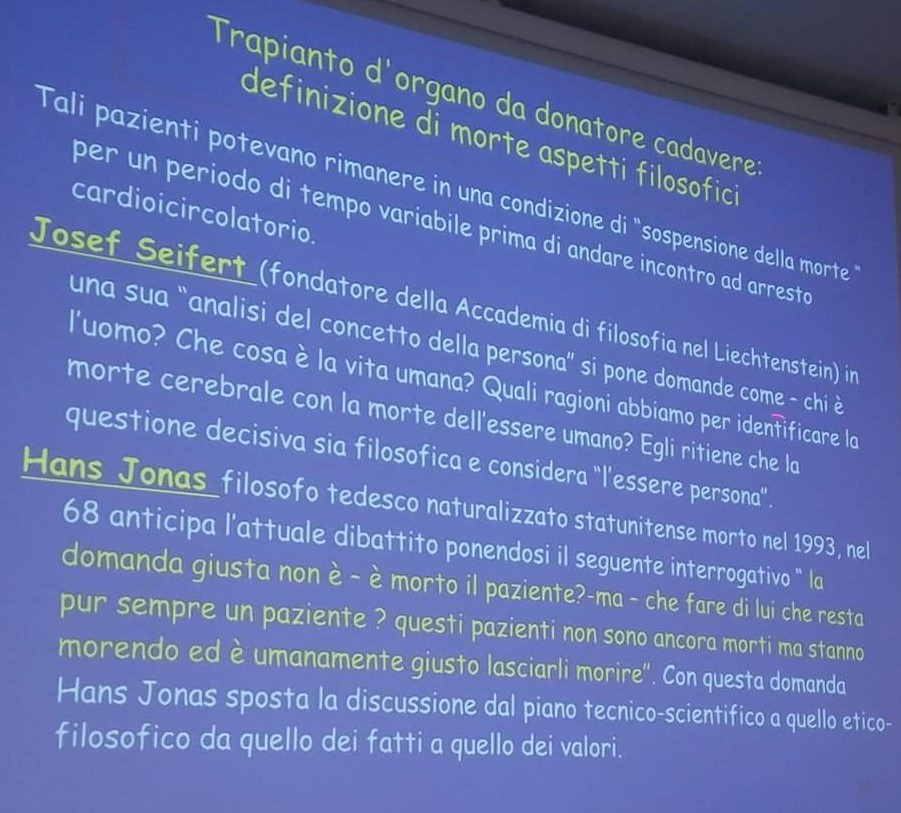
\includegraphics[width=4.80556in,height=3.08451in]{media/image13.emf}

GESTIONE CICLO RIFIUTI (sezione)

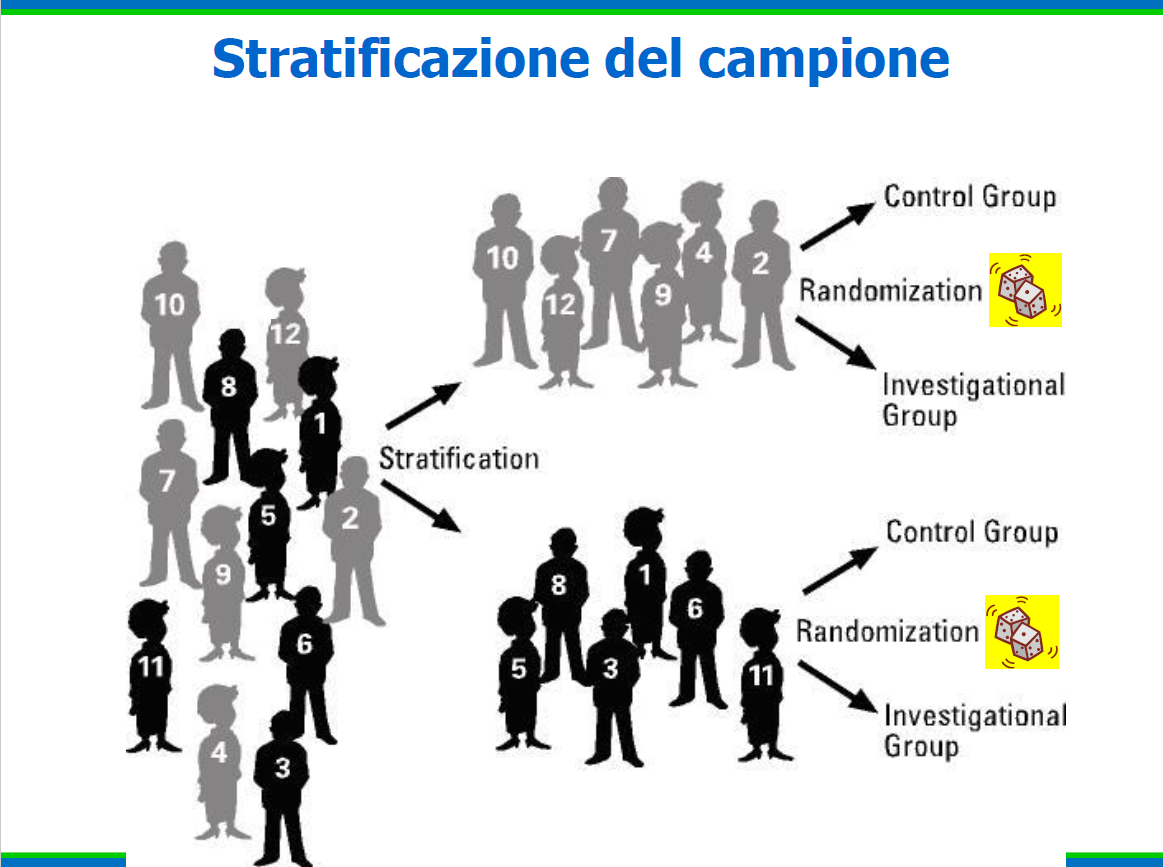
\includegraphics[width=5.39021in,height=3.54876in]{media/image14.emf}

Il tema è quanto mai attuale; oggi i problemi più grossi nella gestione
dei rifiuti sono i seguenti:

\begin{itemize}
\item
  \begin{quote}
  ABBANDONO STRADALE E DISCARICHE ABUSIVE (si pensi all'Italia nel
  complesso)
  \end{quote}
\end{itemize}

\begin{quote}
Per assurdo i sistemi molto fiscali e complicati di raccolta
differenziata di fatto hanno accentuato il problema dell'abbandono dei
rifiuti. Per esempio se si ha necessità di smaltire un materasso si
incontrano diverse difficoltà: dalla mancanza di reperibilità di
informazioni sul corretto smaltimento (non rispondono ai numeri verdi
indicati) alla tassazione sul ritiro del bene; succede spesso che per
esasperazione la gente carichi il materasso in questione e lo abbandoni.
\end{quote}

\begin{itemize}
\item
  \begin{quote}
  ECOMAFIE che gravano su chi gestisce, trasporta e trasforma i rifiuti;
  esse condizionano il mercato, condizionano le scelte e a volte
  bloccano alcune operazioni fatte nell'interesse di una corretta
  gestione dei rifiuti.
  \end{quote}
\item
  \begin{quote}
  STRUMENTALIZZAZIONI: già trattate
  \end{quote}
\item
  \begin{quote}
  EDUCAZIONE DEI CITTADINI: se la raccolta differenziata può
  ragionevolmente arrivare al 70\% (con impegno da parte del singolo ma
  senza impazzire) è incomprensibile come in alcune città dal grande
  senso civico come può essere Parma si arrivi soltanto al 50\%.
  Scendendo in altre parti d'Italia si arriva al 40, al 30 e addirittura
  al 20\% in città che addirittura sono capoluogo di Provincia. Questo
  sta a significare che i cittadini non collaborano a questo tipo di
  attività. Tra il 70\% e il 20\% (o ancora meno) la differenza è che
  viene avviata allo smaltimento (o in inceneritore o in discarica) una
  quantità di rifiuti assolutamente maggiore, di quasi tre volte tanto.
  Il dimensionamento degli inceneritori e delle discariche, che sono i
  due sistemi utilizzati per smaltire la quota residua (quella che non
  viene differenziata), dipende da quanta raccolta differenziata viene
  fatta. A Parma la percentuale di differenziata sta lentamente salendo;
  ci sono altre regioni virtuose come l'Alto Adige dove si è raggiunto
  il 70\%-75\%. La norma nazionale stabilisce un 70\%, la realtà in
  media è sul 40\%.
  \end{quote}
\end{itemize}

Perché si parla di rifiuti oggi?

Solidi e liquidi, il concetto è che da rifiuti non raccolti e non
trattati nel modo corretto possono derivare problemi a livello
ambientale ed effetti sulla salute umana. Il problema della gestione dei
rifiuti è un problema serio, anche per via della estrema difficoltà
nella riduzione della produzione degli stessi.

L'Italia ha fatto una scelta complessiva (in realtà l'Emilia Romagna fa
eccezione perché ha scelto la via degli inceneritori da parecchi anni)
di tenere il numero degli inceneritori basso; si arriva a incenerire una
quota non superiore all'11\% del totale dei rifiuti, con un recupero
medio del 44\% e con l'altro 45\% che finisce ancora oggi in discarica.
È chiaro che l'obiettivo finale è di ridurre la quota indifferenziata,
sia pur con difficoltà, però tenendo presente il valore del 70\% (nato
appunto per tenere conto di questa oggettiva difficoltà nella raccolta
dei rifiuti nonostante il grande impegno collettivo).

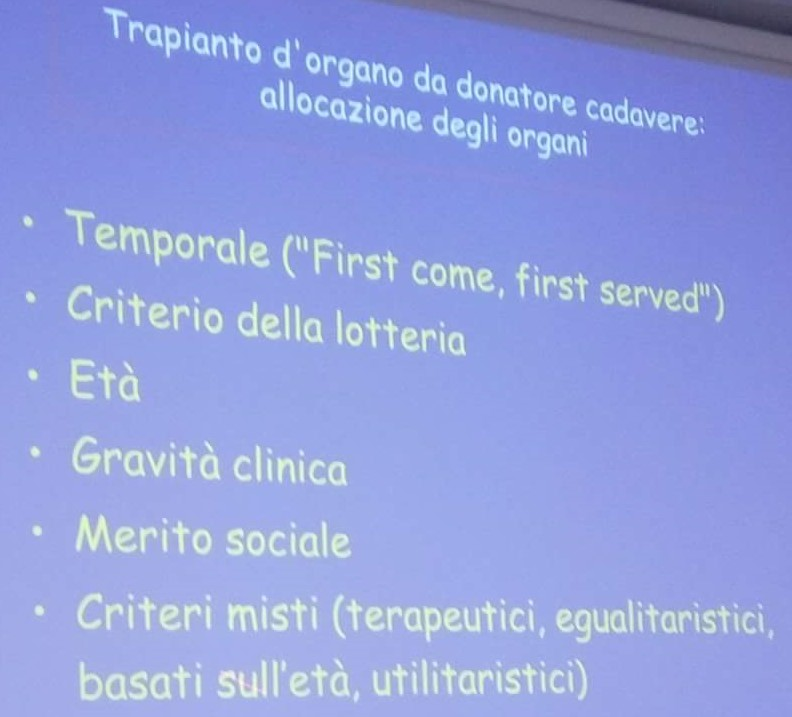
\includegraphics[width=5.99144in,height=4.30409in]{media/image15.emf}

Il nodo cruciale per quanto riguarda la salute umana è la scelta
\textbf{INCENERITORE O DISCARICA?}

Tutti sono d'accordo sulla necessità di aumentare la raccolta
differenziata; l'OMS (e in generale chi affronta il problema dal punto
di vista scientifico) non ha dubbi sul fatto che nel complesso e nel
lungo termine la discarica è peggiore perché si va ad inquinare il suolo
per molti decenni; si tenga conto che un suolo usato come discarica non
può più essere usato per nessun'altra attività. Non si può chiaramente
costruire sopra un terreno che è stato adibito a discarica; al massimo
20 anni dopo si può creare un parco. Per quanto riguarda gli
inceneritori, esistono alcuni effetti provati, ma c'è una sostanziale
tranquillità derivata da una serie di studi che affermano che gli
impianti di nuova generazione apportano un modesto contributo
all'inquinamento dell'aria (modesto contributo non vuol dire zero!). Per
fare un esempio, l'inceneritore di Parma incide per l'1\% sul PM 10
totale dell'area (una percentuale molto bassa rispetto a tutto quello
che sta intorno).

L'impatto sulla salute è ridotto e non rilevabile. Sono d'aiuto i dati
che provengono da uno degli studi più completi mai fatti nel mondo: lo
studio \emph{MONITER}, fatto sulla popolazione che ha vissuto per anni
nei pressi degli inceneritori della regione Emilia Romagna. Esso ha
escluso effetti gravi sulla salute in chi abita o ha abitato vicino agli
inceneritori.

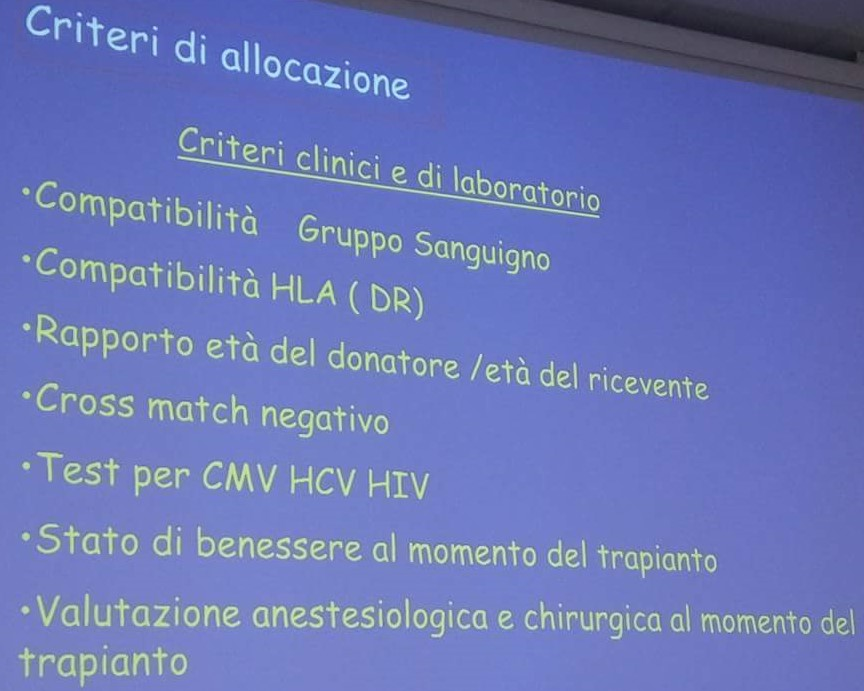
\includegraphics[width=5.98530in,height=3.56442in]{media/image16.emf}

Si osservi che per quanto riguarda l'incidenza dei tumori nelle femmine
nessun dato è statisticamente significativo; per i maschi si è visto che
si ha un aumento di un tumore e una diminuzione di un altro, questo però
è compatibile con la fluttuazione statistica quindi non rilevante
davvero dal punto di vista epidemiologico. La conclusione dello studio
MONITER è stata molto tranquillizzante, soprattutto se si considera il
fatto che sono dati che riguardano inceneritori di vecchia data; gli
impianti di oggi a maggior ragione dovrebbero inquinare ancora meno.

Per la verità lo studio MONITER ha mostrato un possibile più basso peso
alla nascita in chi ha vissuto vicino agli inceneritori; questo dato ha
sorpreso e merita un approfondimento perché può esservi una correlazione
sanitaria tra l'inquinamento dovuto all'inceneritore e quindi di fatto
l'inquinamento atmosferico (è sempre difficile scindere ciò che arriva
dall'inceneritore da ciò che arriva per via del traffico motorizzato o
per via del riscaldamento domestico).

Quali sono i rischi sanitari e ambientali della gestione dei rifiuti?

\begin{enumerate}
\def\labelenumi{\arabic{enumi}.}
\item
  \begin{quote}
  PROBLEMA DI IGIENE E DECORO URBANO legato ai sistemi di raccolta:
  nelle emergenze le città spesso sono impresentabili (chiaramente non
  si tratta di Parma ma di città come Roma o Napoli che hanno spesso
  emergenze rifiuti). Si consideri tuttavia che Roma è l'unica capitale
  europea che non possiede un inceneritore a disposizione; non è sempre
  facile trovare terreni per fare discariche in quanto sono necessarie
  aree ampie, non abitate, in cui i proprietari volontariamente si
  privano del terreno e in cui le amministrazioni garantiscono che quei
  terreni non verranno utilizzati per altro scopo da lì all'eternità di
  fatto. Napoli ha risolto il problema brillantemente caricando i
  rifiuti e mandandoli in Olanda (è una soluzione ma si invita alla
  riflessione)
  \end{quote}
\item
  \begin{quote}
  SICUREZZA DEL PERSONALE INCARICATO ALLA RACCOLTA E AL TRASPORTO DEI
  RIFIUTI: i netturbini sono tra le categorie a rischio per le punture
  con aghi o siringhe
  \end{quote}
\item
  \begin{quote}
  CONTAMINAZIONE DELL'AMBIENTE SOPRATTUTTO LEGATA AI RIFIUTI SPECIALI:
  non è un caso che i rifiuti ospedalieri speciali vengano raccolti con
  un sistema diverso, mandati poi non in discarica ma all'inceneritore e
  solo agli inceneritori autorizzati;
  \end{quote}
\item
  \begin{quote}
  INQUINAMENTO DEL SUOLO E DELLE ACQUE legato alle discariche
  \end{quote}
\item
  \begin{quote}
  INQUINAMENTO DELL'ARIA legato agli inceneritori
  \end{quote}
\item
  \begin{quote}
  EMERGENZE LEGATE ALLA CATTIVA PIANIFICAZIONE di raccolta dei rifiuti.
  \end{quote}
\end{enumerate}

\end{document}
